\documentclass[tikz,border=2pt]{standalone}
\usepackage{amsmath}
\usepackage{amssymb}
\usepackage{xcolor}

\definecolor{journalink}{HTML}{1F1C18}
\definecolor{journalmuted}{HTML}{8A7F72}
\definecolor{journalaccent}{HTML}{9C2D2D}

\begin{document}
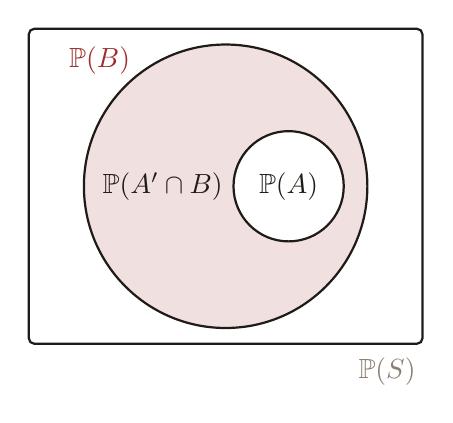
\begin{tikzpicture}[
  x=1cm,
  y=1cm,
  every node/.style={font=\normalsize}
]
  \def\bigcircle{(1,0) circle (1.8)}
  \def\smallcircle{(1.8,0) circle (0.7)}

  \begin{scope}[even odd rule]
    \clip \smallcircle \bigcircle;
    \path[fill=journalaccent, fill opacity=0.15] \bigcircle;
  \end{scope}

  \draw[journalink, line width=0.8pt, rounded corners=2pt] (-1.5,-2) rectangle (3.5,2);
  \draw[journalink, line width=0.8pt] \bigcircle;
  \draw[journalink, line width=0.8pt] \smallcircle;

  \node[journalink] at (0.2,0) {$\mathbb{P}(A^{\prime}\cap B)$};
  \node[journalink] at (1.8,0) {$\mathbb{P}(A)$};
  \node[journalaccent] at (-0.6,1.6) {$\mathbb{P}(B)$};
  \node[journalmuted] at (3.05,-2.35) {$\mathbb{P}(S)$};
\end{tikzpicture}
\end{document}
